\section{Introduction}
\label{sec:intro}


Transformers, in particular decoder-only models (e.g.\ GPT~\citep{brown2020language}, Llama~\citep{touvron2023llama}) which process input sequences in a causal fashion, are one of the main drivers of modern deep learning's success.
Numerous approaches attempt to approximate the core attention layer to address its efficiency issues~\citep{tay2022efficient}, such as scaling quadratically in sequence length during training and requiring a cache of size linear in sequence length during autoregressive generation.
In parallel, a class of alternative sequence models, structured state-space models (SSMs), have emerged with linear scaling in sequence length during training and constant state size during generation.
They show strong performance on long-range tasks (e.g. S4~\citep{gu2022efficiently}) and recently matched or beat Transformers on language modeling (e.g. Mamba \citep{gu2023mamba}) at small to moderate scale.
However, the development of SSMs have appeared disjoint from the community's collective effort to improve Transformers, such as understanding them theoretically as well as optimizing them on modern hardware.
As a result, it is more difficult to understand and experiment with SSMs compared to Transformers, and it remains challenging to train SSMs as efficiently as Transformers from both an algorithmic and systems perspective.


Our main goal is to develop a rich body of theoretical connections between structured SSMs and variants of attention.
This will allow us to transfer algorithmic and systems optimizations originally developed for Transformers to SSMs, towards the goal of building foundation models that perform better than Transformers while scaling more efficiently in sequence length.
A milestone contribution in this direction was the \textbf{Linear Attention (LA)} framework \citep{katharopoulos2020transformers},
which derived a connection between autoregressive attention and linear RNNs
by showing the equivalence between ``dual forms'' of quadratic kernelized attention and a particular linear recurrence.
This duality allows new capabilities such as the ability to have both efficient parallelizable training and efficient autoregressive inference.
In the same spirit, this paper provides multiple viewpoints connecting linear-complexity SSMs with quadratic-complexity forms to combine the strengths of SSMs and attention.%
\footnote{Technically speaking, these connections only relate to certain flavors of attention; the title of this paper is an homage to \citet{katharopoulos2020transformers} which first showed that ``Transformers are RNNs''.}

\iftoggle{arxiv}{
\begin{wrapfigure}{R}{0.48\linewidth}
  \begin{center}
    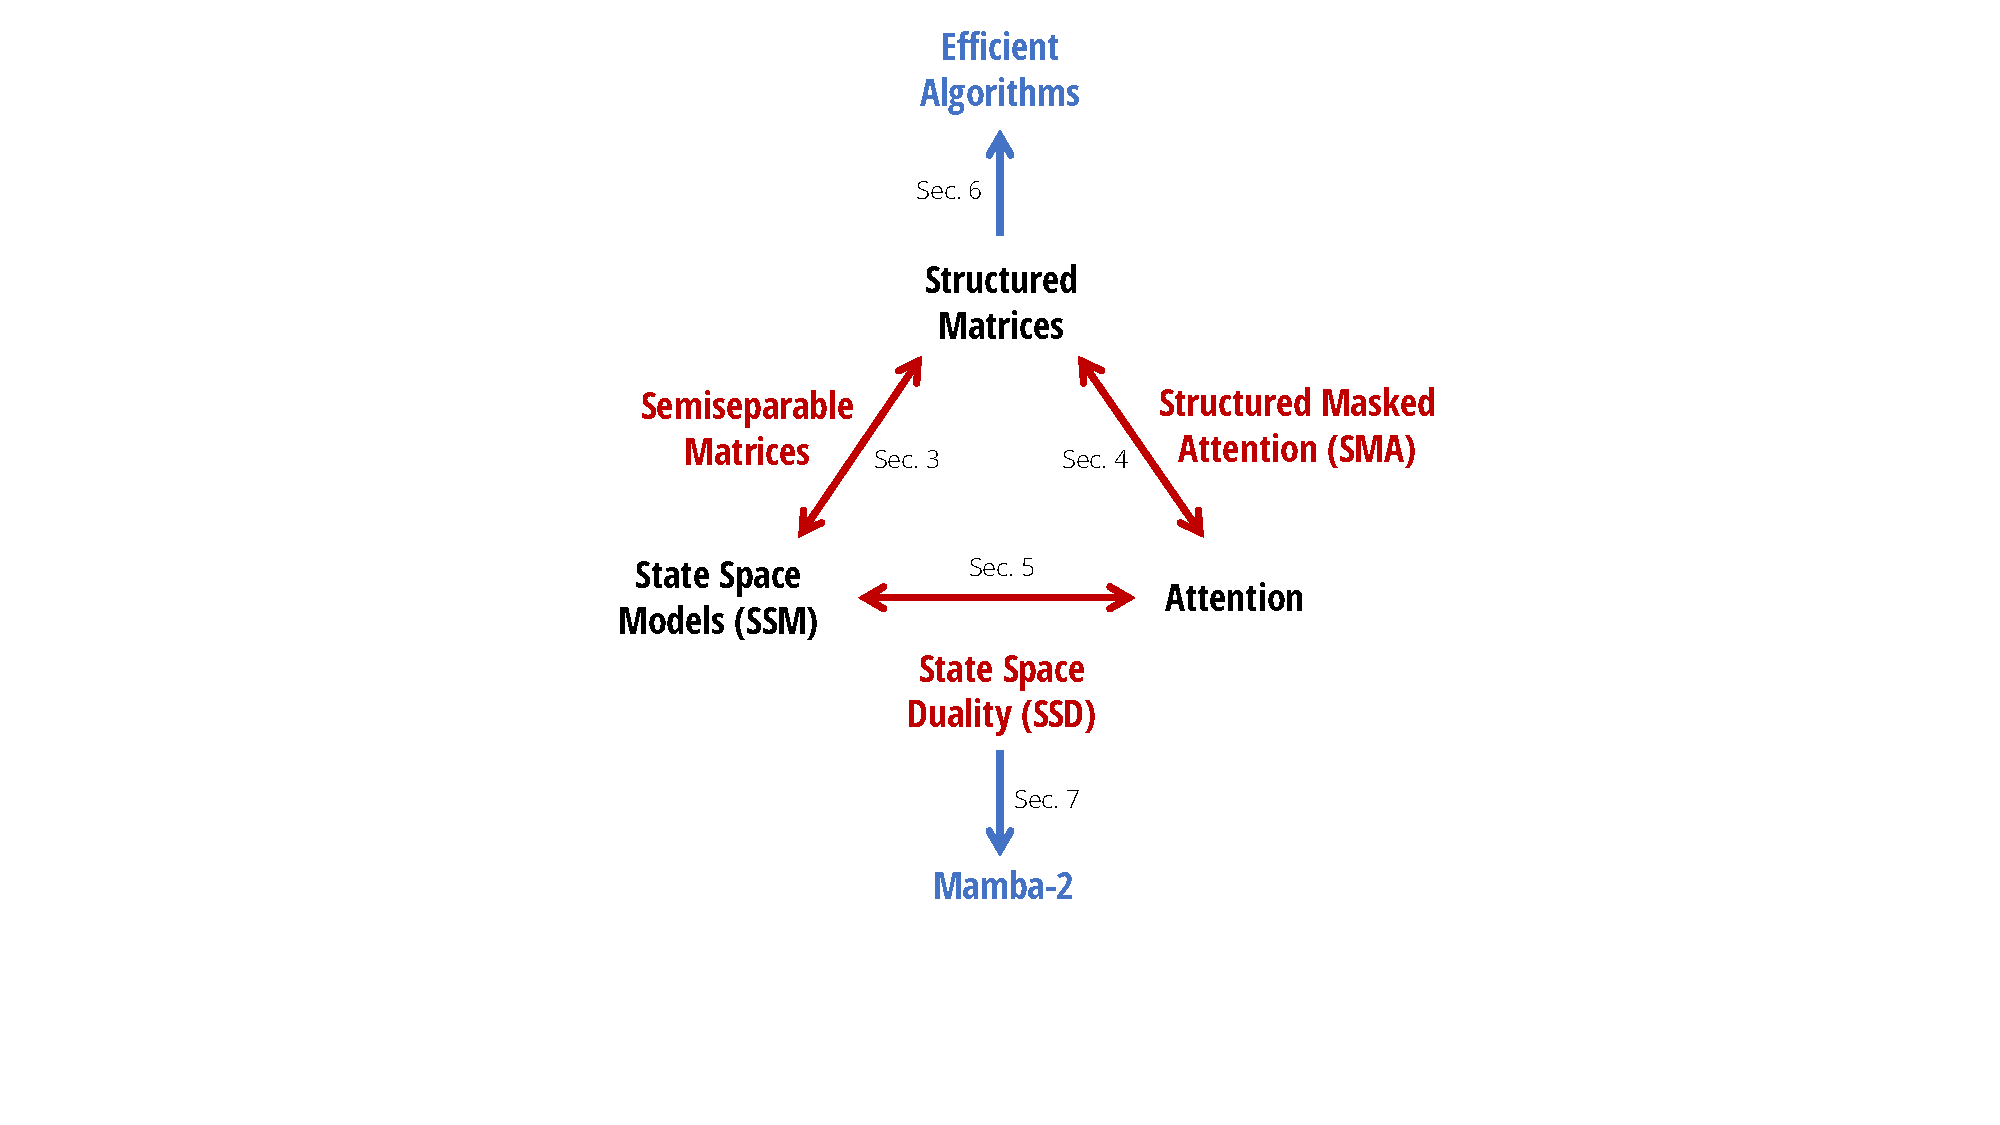
\includegraphics[width=\linewidth]{fig/ssd_roadmap.pdf}
  \end{center}
  \caption{
    (\textbf{Structured State-Space Duality}.)
    This paper fleshes out the relationship between state space models and attention through the bridge of structured matrices.
  }
  \label{fig:roadmap}
\end{wrapfigure}
}{}

\para{State Space Duality.}
Our framework connecting structured SSMs and variants of attention, which we call \textbf{structured state space duality} (SSD),
is made through the abstractions of \textbf{structured matrices}:
matrices with subquadratic parameters and multiplication complexity.
We develop two broad frameworks for representing sequence models, one as matrix transformations and one as tensor contractions, which each reveal different perspectives of the duality.
Our technical contributions include:
\begin{itemize}[leftmargin=*,itemsep=0pt,topsep=0pt]
  \item We show an equivalence between state space models and a well-studied family of structured matrices called \textbf{semiseparable matrices}\iftoggle{arxiv}{ (\cref{sec:ssm})}{}.
    This connection is at the heart our framework, revealing new properties and algorithms for SSMs. A central message of this paper is that \emph{different methods of computing state space models can be reframed as various matrix multiplication algorithms on structured matrices}.
  \item We significantly improve the theory of linear attention~\citep{katharopoulos2020transformers}.
    We first provide an incisive proof of its recurrent form through the language of tensor contractions, and then generalize it to a new family of \textbf{structured masked attention (SMA)}\iftoggle{arxiv}{ (\cref{sec:attention})}{}.
  \item We connect SSMs and SMA, showing that they have a large intersection that are duals of each other, possessing both SSM-like linear and attention-like quadratic forms\iftoggle{arxiv}{ (\cref{sec:ssd})}{}.
    \iftoggle{arxiv}{We also prove that any kernel attention method possessing a fast recurrent form must be an SSM.}{}
\end{itemize}


Beyond its intrinsic theoretical value, our framework opens up a broad set of directions for understanding and improving sequence models.

\para{Efficient Algorithms.}
First and most importantly, our framework exposes new efficient and easily-implementable algorithms for computing SSMs\iftoggle{arxiv}{ (\cref{sec:efficient})}{}.
We introduce a new \textbf{SSD algorithm}, based on block decompositions of semiseparable matrices, that takes advantage of both the linear SSM recurrence and quadratic dual form, obtaining optimal tradeoffs on all main efficiency axes (e.g. training and inference compute, memory usage, and ability to leverage matrix multiplication units on modern hardware).
A dedicated implementation of SSD is $2-8\times$ faster than the optimized selective scan implementation of Mamba, while simultaneously allowing for much larger recurrent state sizes ($8\times$ the size of Mamba or even higher, with minimal slowdown).
SSD is highly competitive with optimized implementations of softmax attention (FlashAttention-2~\citep{dao2023flashattention2}), crossing over at sequence length 2K and 6$\times$ faster at sequence length 16K.


\iftoggle{arxiv}{
\para{Architecture Design.}
One major obstacle to adopting new architectures such as SSMs is the ecosystem tailored to Transformers, such as hardware-efficient optimization and parallelism techniques for large-scale training.
Our framework allows using established conventions and techniques for attention to build a vocabulary of architecture design choices for SSMs, and further improve them (\cref{sec:architecture}).
For example, we introduce the analog of heads from multi-head attention (MHA) to SSMs.
We show that the Mamba architecture is a \textbf{multi-input SSM (MIS)} that turns out to be analogous to \textbf{multi-value attention (MVA)}, and compare other variants of Mamba with different head structures.

We also use these ideas to make slight modifications to the Mamba block, which allows tensor parallelism to be implemented (e.g. in the style of Megatron~\citep{shoeybi2019megatron}).
The main ideas include introducing grouped-value attention (GVA) head structure, and moving all data-dependent projections to occur in parallel at the beginning of the block.


}{
  \para{Mamba-2.}
  Additionally, inspired by the connection between SSMs and Transformers, we slightly modify the neural network architecture of Mamba by moving all data-dependent projections to occur in parallel at the beginning of the block. %
}
The combination of the modified parallel Mamba block, together with using SSD as the inner SSM layer, results in the \textbf{Mamba-2} architecture.
We investigate Chinchilla scaling laws for Mamba-2 in the same setting as Mamba, finding that it Pareto dominates Mamba and Transformer++ in both perplexity and wall-clock time.
We additionally train a family of Mamba-2 models at varying sizes on the Pile, showing that it matches or outperforms Mamba and open source Transformers on standard downstream evaluations.
For example, Mamba-2 with 2.7B parameters trained on 300B tokens on the Pile outperforms Mamba-2.8B, Pythia-2.8B and even Pythia-6.9B trained on the same dataset.

\iftoggle{arxiv}{
\paragraph{Systems Optimizations.}
The SSD framework connects SSMs and Transformers, allowing us to leverage a rich body of work on systems optimizations developed for Transformers~(\cref{sec:systems}).
\begin{itemize}[leftmargin=*,itemsep=0pt,topsep=0pt]
  \item For example, Tensor Parallelism (TP) is an important model parallelism technique to train large Transformer models by splitting each layer across GPUs on the same node.
    We design Mamba-2 to be TP-friendly, reducing the number of synchronization point per block by half.
  \item For very long sequences whose activations do not fit on one device, sequence parallelism has been developed for the attention blocks.
    We describe how to train SSMs in general and Mamba-2 in particular with sequence parallelism, by passing the recurrent states between devices.
  \item For finetuning with examples of different lengths, for best efficiency, Transformer requires sophisticated techniques to remove padding tokens and perform attention on variable length sequences.
    We show how Mamba-2 can be trained with variable sequence lengths efficiently, requiring no padding tokens.
\end{itemize}
}{}

\cref{sec:experiments} empirically validates Mamba-2 on language modeling, training efficiency, and a difficult multi-query associative recall task~\citep{arora2024simple}.
Finally, in \cref{sec:related}, we provide an extended related work and discuss potential research directions opened up by our framework.

Model code and pre-trained checkpoints are open-sourced at \url{https://github.com/state-spaces/mamba}.





